\section{Summary} \label{sec:summary}

\subsection{Applicability and Limitations}

- Density ranges, temperature ranges, optically thin condition

- Remind reader that cooling lengths are potentially very short and
having a fancy model is perhaps not very relevant at 1kpc
resolution. Can give some guidance of how to apply this.

\begin{figure*}
  \centering
  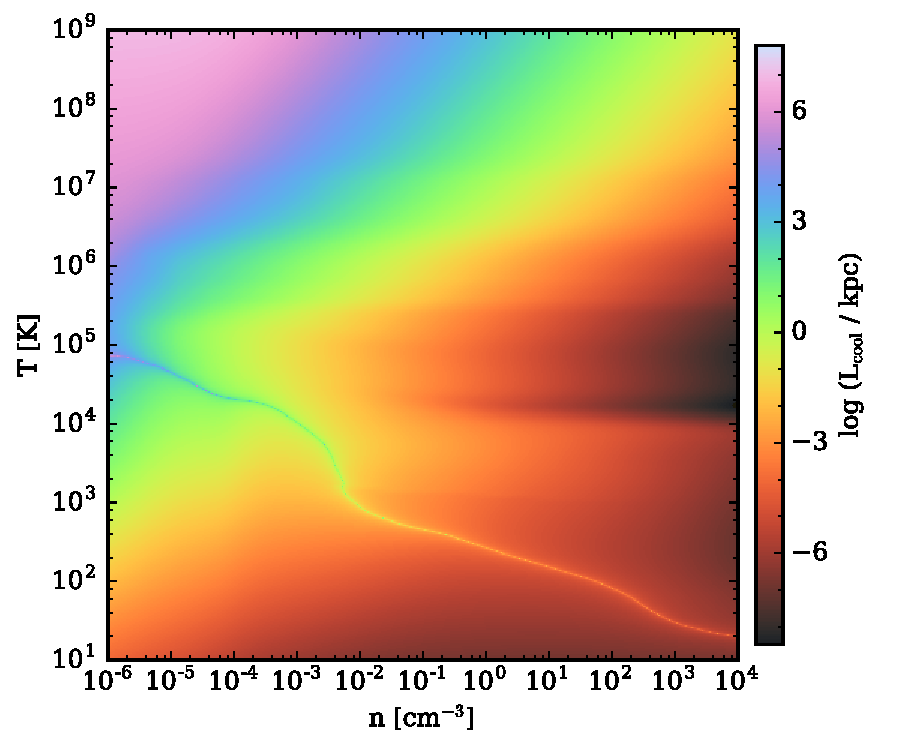
\includegraphics[width=0.84\textwidth]{cooling_length.pdf}
  \caption{
    The cooling length, defined as the product of the Jeans length and
    the cooling time, as a function of number density and temperature
    for a gas with solar metallicity exposed to a radiation field
    defined by the model of \citet{2012ApJ...746..125H} at z = 0.  The
    narrow line extending from the middle, left to the bottom, right
    represents the temperature where heating and cooling are
    balanced.  Above this line, the gas is being cooled while below
    the line it is being heated.
  } \label{fig:cooling-length}
\end{figure*}

\subsection{codes which have Grackle implementations}


\subsection{Future Directions} \label{Future_Directions}

\subsubsection{Future API changes} 
Replace the 18 array pointers to a single pointer to a struct of arrays?

\subsubsection{Including new rates and models in Grackle}
\jr{} The current code structure is highly integrated. This makes introducing new rates for the 
chemical network or cooling network a rather intricate task requiring multiple changes throughout the code. 
Apart from the fact that this is more time consuming it is also much more error prone. In a future release of the 
code the modularity of the code will be increased greatly. There will be a function to populate the species 
rate coefficients and a function to populate the cooling coefficients. Seperate template files can then be 
updated by a developer wishing to use their own rates. This file can then be included in the build and a flag
set to indicate the new rates be used in place of the old rates. Furthermore, a similar method will be 
implemented for solving the network. A template network solver will be available which the developer can use to 
implement a new network with a developer determined number of species. The developer will be responsible for
updating only three files to achieve a solution to their own chemical network. 

\subsubsection{Connection to Radiative Transfer}

\subsubsection{Multiple element cooling}

\subsubsection{Other heating sources?}
